\documentclass{article}
\usepackage[utf8]{inputenc}

\title{Conversion of Analog to Spiking Transformer Networks}
\author{Viktor Studenyak\\[0.5cm]{Advisor: Etienne Müller}}
\date{\small March 2021}

\usepackage{natbib}
\usepackage{graphicx}
\usepackage{hyperref}
\usepackage{natbib}
\usepackage{subfig}
\graphicspath{{images/}}
\bibliographystyle{apalike}

\begin{document}

\maketitle

\section{Introduction}

Transformer Networks revolutionized the field of natural language processing. They are able to model temporal sequences very well, achieving remarkable performance in machine language translation \cite{transformer}. Transformers adapted for computer vision operating on image patches have shown excellent performance on many datasets, at the same time being less computationally expensive \cite{vision_transformer}. On the other hand, recent developments in neuromorphic hardware give an opportunity for energy-efficient computations. The limitation is, that neuromorphic hardware is well suited for spiking neural networks, but not for more conventional artificial neural networks. Conversion of trained ANNs into SNNs yielded best results \cite{snn_overview}  and serve as a  benchmark for SNN performance for fully-connected and convolutional neural networks \cite{dl_in_snn}.

In this work, we introduce the spiking architecture for self-attention-based Transformer networks obtained through weight conversion using weight normalization tools proposed by \cite{rueckauer2016theory}.

\section{Related Works}
There are two major approaches for training networks of spiking neurons: unsupervised learning using spike-timing-dependent plasticity \cite{unsupervised_stdp} and supervised learning using backpropagation \cite{snn_backpropagation}. Other works on supervised learning with backpropagation are \cite{supervised_temporal_coding}, \cite{event_driven_backprop}, \cite{slayer}, \cite{surrogate}, which propose techniques for overcoming continuous-value nature of backpropagation algorithm.

On the other hand, conversion methods show superior performance in comparison with the previously described methods. By utilizing the non-negativity property of ReLU activation functions, the average neuron firing rate can be approximated \cite{conversion_first}. This method was neglecting bias and was not particularly good for activations with comparably greater values, than the weights. In subsequent work, \cite{diehl_fast_classifying} proposed a weight normalization algorithm, which involved activations of neurons for scaling factor estimation. \cite{rueckauer2016theory} proposed a way to make weight normalization more robust to very large outliers to avoid simulation latency in the network of spiking neurons. In \cite{conversion_continuous_valued} methods for max-pooling and batch normalization layer conversion were proposed. More recent methods proposed architectures for the conversion of more complex architectures, such as deep residual networks \cite{hu2020spiking}, \cite{deeper_spiking} and YOLO-architecture \cite{kim2019spikingyolo}. 

\begin{figure}[b!]
\begin{center}
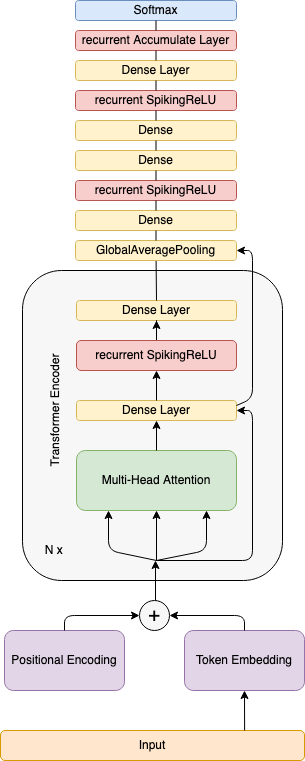
\includegraphics[width=0.4 \textwidth]{SpikingTransformer.png}
\caption{Spiking Transformer architecture}
\label{fig:transformer}
\end{center}
\end{figure}


In \cite{hybrid_conversion} even went further and combined the ann to snn weight conversion as initialization phase with the spike-based backpropagation and achieved superior results in terms of simulation latency and accuracy compared to ann-snn conversion methods or conventional spiking training methods, such as surrogate gradient or spike-based backpropagation.

In this work, we propose spiking transformer architecture, solving two problems: natural language processing in form of sentiment analysis and image classification for written digit recognition.


\section{Methodology}
\textbf{Architecture}. Network architectures with dense layers with ReLU activation functions are trained. In the spiking architecture, those layers are converted to dense layers without activation in combination with a recurrent layer with SpikingReLU as recurrent cells. In this combination, layers simulate the behavior of fire-integrate neurons. A dense layer with softmax activation at the tail of the network is converted to a dense layer in combination with a recurrent layer with Accumulate as recurrent cells. Accumulate cells are aggregating values over the simulation timesteps. SpikingReLUs use the reset by subtraction method to reset membrane potential, it has shown better efficiency for conversion of networks of spiking neurons \cite{conversion_continuous_valued}. The overall architecture for the NLP Transformer network is shown in Figure \ref{fig:transformer}.

\begin{figure}[b!]
\begin{center}
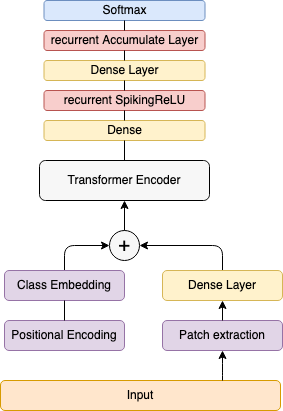
\includegraphics[width=0.5 \textwidth]{SpikingVisionTransformer.png}
\caption{Spiking Vision Transformer architecture}
\label{fig:vision_transformer}
\end{center}
\end{figure}

\textbf{Weight normalization}. For weight normalization, we use the robust data-based normalization method proposed by \cite{rueckauer2016theory}. We take a subset of a test set and compute activations for the layers that have to be converted (layers with ReLU activation function) and get its p-th percentile value. First, we compare maximal values of bias and weight for this layer and pick a greater value. Then, we compare this value with a maximal value of activation and pick a greater value. This value is then divided by the scaling factor of the previous converted layer. Finally, we rescale weights of the layer using the previously computed scaling factor. We also rescale bias with respect to the current scaling factor, not discounting it with the scaling factor of the previous layer.

\section{Experiments}

\begin{figure}
\centering
    \begin{subfigure}
      \centering
      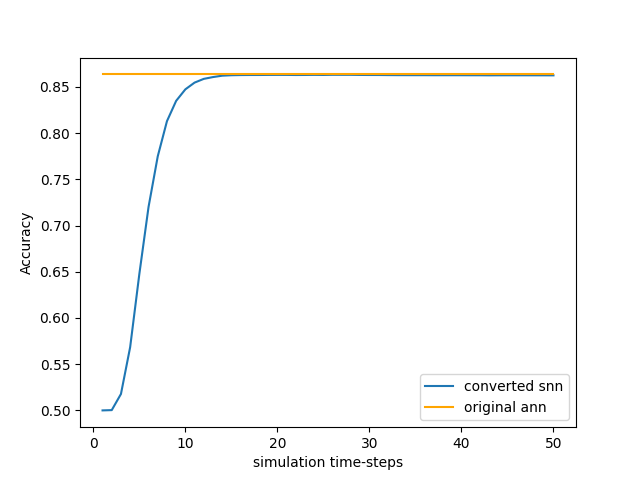
\includegraphics[width=0.7\linewidth]{assets_simulated_accuracy_nlp_v2.png}
      \caption[width=.4\linewidth]{Simulation accuracy of NLP transformer}
      \label{fig:sub1}
    \end{subfigure}
    \begin{subfigure}
      \centering
      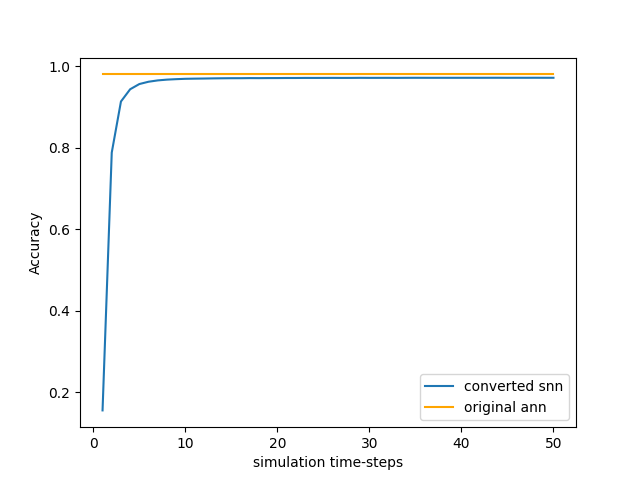
\includegraphics[width=0.7\linewidth]{assets_simulated_accuracy_vit_v2.png}
      \caption{Simulation accuracy of vision transformer}
      \label{fig:sub2}
    \end{subfigure}
\label{fig:test}
\end{figure}

\textbf{Datasets}. We train and evaluate NLP Transformer Network on IMDB movie review sentiment classification dataset \cite{imdb_dataset}. The dataset includes 25.000 reviews from IMDB, each review has one label, positive or negative sentiment. Dataset is split into two halves, one half is used for training, another one for testing.

For the first experiment, we use a vocabulary size of 20.000, which means that only the top 20.000 words will be considered. We also crop reviews to a maximal length of 200 words, reviews that have fewer words will be filled with zero paddings. We transform labels to categorical vectors, which can have two states: positive or negative. We do not represent reviews as one-hot encoded vectors but as sequences of encoded words. We use embedding layers for the word sequences and also for encoding positions of the words. Then, we add token embeddings to positional embeddings, which then are fed to the multi-head self-attention module.

In our second experiment, we use a vocabulary size of 500 and a maximal length of reviews of 50. Similar to the first experiment, we crop reviews to maximal length and fill reviews with zeros, if they don't have enough words. We represent words as one-hot encoded vectors.

Our vision Transformer Network we train and evaluate on MNIST dataset. It consists of 60.000 images for the training and 10.000 for the testing phase. For vision transformer, we use architecture proposed by \cite{16x16words}.

\textbf{Experiment 1. NLP Transformer.} We have built a network similarly to \cite{transformer} illustrated by Figure 1. For details please refer to \ref{fig:transformer}. We use embedding over a range of numbers to get positional encoding. We add positional encoding to the token embedding of the input. The transformer encoder part is equivalent to the original transformer, except the dense layer with ReLU as an activation function. We exchange it as previously mentioned with a dense layer without any activation function and a recurrent layer with SpikingReLU as a recurrent cell. After the transformer encoder part, we use the global average pooling layer. Subsequently, we exchange every dense layer with activation function by the dense layer without activation function followed by recurrent layer. We also exchange the final layer with the softmax activation function by recurrent layer with accumulation cell followed by softmax operation.

\textbf{Experiment 2. Vision Transformer.} For this experiment we have built a network similarly to \cite{16x16words}. The exact architecture is shown in Figure 2. We divide every image into four patches, each patch consists of 7x7 pixels. We then flatten the patch and make a linear projection of all patches. We add positional encoding together with class embedding to linear projections of the patches. The transformer encoder part of the network is very similar to the encoder part of the NLP transformer. We also flatten the output of the transformer encoder instead of picking the zeroth dimension, which is different from the original vision transformer.

For both experiments, we train the ANN network 50 times and then simulate each ANN for 50 timesteps to average out the results for different random seeds. 
For the NLP transformer, we train the network for 2 epochs with a batch size of 64 and achieve the averaged accuracy of the ANN network of 86.36 percent. On a converted network after 50 simulation steps, we achieve an accuracy of 86.25 percent, which yields a conversion loss of 0.11 percent. On the other hand, we achieve an accuracy of 86.1 percent after only 13 timesteps.
For the vision transformer, we train the network for 2 epochs with a batch size of 64 and achieve an averaged accuracy of an ANN network of 97.99 percent. Although we achieve an average result of 97.16 after 50 timesteps on a converted network, we achieve a result of 97.02 only after 13 timesteps. Conversion loss is 0.83 percent for the converted network after 50 timesteps.


\section{Discussion}
In this work, we introduced the novel conversion of transformer architectures from deep artificial networks to networks of spiking neurons. We obtained architectures with near loss-less conversion: 0.11 percent for NLP transformer and 0.83 percent for vision transformer.

For future work, several directions can be chosen. On the one hand, the existing architectures of ann-snn conversion can be further explored, e.g. run on more datasets, apply to more advanced datasets, perform a hyperparameter search or try out the architecture on the neuromorphic hardware. On the other hand, it could be interesting to apply similar techniques to more recent and advanced types of transformers such as \cite{performer} or \cite{linformer}, which try to reduce the space and time complexity of self-attention mechanism. Another very interesting direction is to explore the hybrid learning approach proposed by \cite{hybrid_conversion} for the transformer networks.


\bibliography{references}
\end{document}
